\chapter{Methodology}


Throughout this section, we provide an in-depth description of the full guidance, navigation, control, and learning architecture that was used during this work. While reading the following subsections, please refer back to figure \ref{fig:Training_Flowchart}, which offers a compact visualization of the whole training loop:


\begin{figure}[H]
    \centering
    
\includegraphics[width=1.0\linewidth]{Figures/Training_Improved_Flattened.jpg}
    \caption{Diagram showing the \acs{parlpo} algorithm's learning loop within the \acs{gnc} architecture constrained by the \acs{ekf} and the classical \acs{cbfqp} controller. A full-page version of this diagram is provided in Appendix~\ref{app:full_page_flowcharts} as Figure~\ref{fig:Training_Flowchart_appendix}.
    }
    \label{fig:Training_Flowchart}
\end{figure}




\section{State, action, and observation.}
\label{sec:state-action-observation}


Consider two agents described in chapter \ref{chap:Problem_Formulation}, a defender which we refer to as player/agent \#1 and an attacker which we refer to as player/agent \#2. These agents evolve under discretized dynamics (e.g., \acs{hcw} or Elliptical), relative to a chief orbit, with a discrete time sampling \(\Delta t\).
For each agent \(i\in\{1,2\}\), their state is defined as:


\[
\mathbf{x}_i =
\begin{bmatrix}
\mathbf{p}_i\\
\mathbf{v}_i
\end{bmatrix}\in\mathbb{R}^{2D},\quad
\mathbf{x}_i^+ = A_d\mathbf{x}_i + B_d\mathbf{u}_i,\quad\mathbf{u}_i\in\mathbb{R}^{D}
\]

where \(p_i,v_i\in\mathbb{R}^{D}\) are the agents position and velocity in the relative frame and \(u_i\) is a commanded acceleration clipped to a system actuation bound \(\|u_i\|_\infty\le u_{\max}\).
With this in mind, the concatenated state for the environment is defined as \(s=\big[x_1^\top,\,x_2^\top\big]^\top\in\mathbb{R}^{4D}\).

We also define $\mathbf{c}$, which denotes the position of the central protected asset about which the spherical arena is defined and which, throughout this work, sits at the chief of the orbit.

Each policy, observes a fixed, task-shaped observation vector defined as:

\begin{equation}
\label{eq:Full_Obs_Both_Agents}
\boxed{
\mathbf{o} =
\begin{bmatrix}
\mathbf{p}_1-\mathbf{c}\\
\mathbf{p}_2-\mathbf{c}\\
\mathbf{p}_2-\mathbf{p}_1\\
\mathbf{v}_1\\
\mathbf{v}_2
\end{bmatrix}
}
\end{equation}



Which for the partially observable settings become the following for the defender:

\begin{equation}
\label{eq:EKF_Obs_Agent_1}
\boxed{
\mathbf{o}_{1,EKF} =
\begin{bmatrix}
\mathbf{p}_1-\mathbf{c}\\
\tilde{\mathbf{p}}_{2,1}-\mathbf{c}\\
\tilde{\mathbf{p}}_{2,1}-\mathbf{p}_1\\
\mathbf{v}_1\\
\tilde{\mathbf{v}}_{2,1}
\end{bmatrix}
}
\end{equation}

And the following for the attacker:

\begin{equation}
\label{eq:EKF_Obs_Agent_2}
\boxed{
\mathbf{o}_{2,EKF} =
\begin{bmatrix}
\tilde{\mathbf{p}}_{1,2}-\mathbf{c}\\
\mathbf{p}_2-\mathbf{c}\\
\mathbf{p}_2-\tilde{\mathbf{p}}_{1,2}\\
\tilde{\mathbf{v}}_{1,2}\\
\mathbf{v}_2
\end{bmatrix}
}
\end{equation}

Where the quantities with tilde are those measured via the bearings-only \acs{ekf} described later in algorithm \ref{alg:kf-methodology}. 

For the fully observable setting, we model the proposed zero-sum game as a discrete-time Markov Decision Process, or \acs{mdp} for short (\cite{Howard1960DynamicProgramming}). Here, the state consists of the previously laid out spacecraft states, the action is the agents' commanded control in 3D, and the transition map is provided and filtered by the spacecraft dynamics and the \acs{cbfqp} controller logic. The reward function and termination conditions are defined by the game's objectives as described in section \ref{sec:Rewards/Termination}. For the partially observable setting, the full-state \acs{mdp} becomes a partially observable version of the same problem, where the agents act based on the bearings-only \acs{ekf} measurements they can get of their opponent instead of having access to its full state.

One future area for development on the partial observability setting would be the implementation of a self-estimation model from which each agent also has to estimate their own position in space (e.g., using an \acs{imu} model), which would add another layer of realism to the research presented in this work. Given the already high degree of complexity of the current research, we decided to not pursue that direction in this work.


\section{Reward shaping and termination conditions}
\label{sec:Rewards/Termination}

The reward function used during learning is designed to guide each agent toward its objectives in the game. The attacker is rewarded for approaching the protected asset, whereas the defender is rewarded for approaching and docking with the attacker. Appropriate termination bonuses and penalties are then applied depending on whether either agent succeeds at completing its objective. In order to define these reward terms, we first construct normalized distance measures based on each agent's position relative to the arena chief and relative to the opposing agent. Normalizing these distances is necessary, as it helps stabilize learning.

We gather the distances of each agent to the center and their relative distance, and normalize them relative to the radius of the spherical arena \(R\) and a constant collision radius \(r_{\text{collision}}\). We use these to define the unitless defender-to-center \(d_1\), attacker-to-center \(d_2\), and docking distance \(d_{\text{dock}}\). Upon normalization, these quantities become:

\[
d_1 = \frac{\|\mathbf{p}_1-\mathbf{c}\|^2}{R^2},\qquad
d_2 = \frac{\|\mathbf{p}_2-\mathbf{c}\|^2}{R^2},\qquad
d_{dock} = \frac{\max(0, \|\mathbf{p}_2-\mathbf{p}_1\| - r_{collision})}{R}
\]



Note that unitless quantity $d_{\text{dock}}$ is not squared unlike unitless quantities $d_1$ and $d_2$ on purpose, as during our game it is meant to be a correcting factor, and $d_1$ and $d_2$ are supposed to be the dominating terms. 

Using these, we finally define our reward function for each time step, which for the defender is simply defined as:

% \[
% \boxed{
% \begin{aligned}
% r_1
% = {}&
% \underbrace{k_{\text{pos}}\, d_2}_{\substack{\text{encourage}\\\text{attacker}\\\text{away from}\\\text{asset}}}
% -
% \underbrace{k_{\text{dock}}\, d_{\text{dock}}}_{\substack{\text{penalize}\\\text{large}\\\text{defender--attacker}\\\text{separation}}}
% \end{aligned}
% }
% \]

\begin{equation}
\label{eq:defender_step_reward}
\boxed{
\begin{aligned}
r_1
= {}&
\underbrace{k_{\text{pos}}\, d_2}_{\substack{\text{encourage attacker}\\\text{away from}\\\text{asset}}}
-
\underbrace{k_{\text{dock}}\, d_{\text{dock}}}_{\substack{\text{penalize large}\\\text{defender--attacker}\\\text{separation}}}
\end{aligned}
}
\end{equation}


% \[
% \boxed{
% \begin{aligned}
% r_1
% = {}&
% \underbrace{k_{\text{pos}}\, d_2}_{\text{encourage attacker away from asset}}
% \end{aligned}
% }
% \]

And with episodic terminal rewards defined as:

\begin{itemize}
    \item $r_1$ += $\beta_{intercept}$ for intercepting/docking to the attacker.
    \item $r_1$ += $\beta_{wall}$ for forcing the attacker out of the spherical arena.
    \item $r_1$ -= $\beta_{intercept}$ for defender crashing onto the asset of interest.
    \item $r_1$ -= $\beta_{wall}$ for defender leaving the spherical arena.
    
\end{itemize}

And in order to keep the game as a min-max zero sum, the attacker reward is simply: 

\[
\boxed{
\begin{aligned}
r_2
= {}&
\underbrace{-r_1}_{\text{attacker reward function}}
\end{aligned}
}
\]

So laid out this turns out to be a reward function in the form:

\begin{equation}
\label{eq:attacker_step_reward}
\boxed{
\begin{aligned}
r_2
= {}&
\underbrace{-k_{\text{pos}}\, d_2}_{\substack{\text{encourage attacker}\\\text{towards}\\\text{asset}}}
+
\underbrace{k_{\text{dock}}\, d_{\text{dock}}}_{\substack{\text{reward large}\\\text{defender--attacker}\\\text{separation}}}
\end{aligned}
}
\end{equation}

And with episodic terminal rewards defined as:

\begin{itemize}
    \item $r_2$ -= $\beta_{intercept}$ for intercepting/docking to the attacker.
    \item $r_2$ -= $\beta_{wall}$ for forcing the attacker out of the spherical arena.
    \item $r_2$ += $\beta_{intercept}$ for defender crashing onto the asset of interest.
    \item $r_2$ += $\beta_{wall}$ for defender leaving the spherical arena.
    
\end{itemize}

\subsection{Partial observability with full-state reward evaluation}
\label{subsec:partial-observability-full-state-rewards}

One must note that the partially observable policies corresponding to observations \ref{eq:EKF_Obs_Agent_1} and \ref{eq:EKF_Obs_Agent_2} also have access to this form of a full-state reward during training. In this setup, the policies act on measurement-based observations, while the reward and terminal conditions are evaluated using the true simulated state.

In this process, we essentially create measurement-based policies that learn from fully observable reward signals, with the intent of recovering behavior similar to the full-state policies despite the sensor noise.

This process proves to be perhaps the simplest way to match sensor measurements to \acs{rl} rewards, which is why it was chosen. There are other potential methods for training partially observable policies, such as behavior-cloning or \acs{dagger}-style imitation learning (e.g., \cite{ross2011reduction}) and distillation-based methods (e.g., \cite{bajcsy2024learning}). We looked into implementing these methods earlier on, but found them to be too computationally expensive, so we proceeded with this full-state reward evaluation setup.



\section{Single Phase \acs{ppo} Algorithm}
\label{sec:single-phase-ppo}

We collect on-policy results via the \acs{ppo} algorithm, based on the foundational work by \cite{schulman2017ppo} and adapted to our dynamics and environment models.

\acs{ppo} was selected for this task as it is a proven, practical, and stable on-policy method for continuous control problems. Compared to other on-policy \acs{rl} algorithms, \acs{ppo} is also relatively straightforward to implement and tune, which proved to be true when we implemented it within the problem setting for our constrained two-player orbital training environment. Plus, given its popularity in \acs{rl} research, there is plenty of documentation on when and how it can be useful.

The benefit of on-policy algorithms like \acs{ppo} compared to off-policy or model-based \acs{rl} methods is that on-policy algorithms train from purpose-made trajectories collected during training. On the other hand, off-policy and model-based \acs{rl} methods rely more on previously existing data, which can be brittle if environments are non-linear, sensitive to mismatches in the training dataset, or if the training data is simply impossible to obtain.

In the fully observable setting, \acs{ppo} is applied over the Markov Decision Process (\acs{mdp}) induced by the orbital game, where each policy update is built from state-action-reward transitions collected from training rollout trajectories. In the partially observable setting, the same overall framework is used, but each agent relies on the measurements of their opponents as opposed to having access to their full state.


Being an on-policy method, \acs{ppo} relies on taking large batches of training data to train its policies. Here, the batches are a fixed length from \(N\) vectorized environments, each of length \(H\), and hence yielding \(B=NH\) transitions per update on each policy. Algorithm \ref{alg:ppo_full_obs} describes the single-phase \acs{ppo} training with full-state observations, whereas algorithm \ref{alg:ppo_kf_on} describes the modifications that are made to the latter when doing partial-observability training with the bearings-only \acs{ekf} measurements: 


\begin{algorithm}[H]
\caption{Single-Phase \acs{ppo} Update with Full-State Observations}
\label{alg:ppo_full_obs}
\begin{algorithmic}[1]
\Require Learning role $r\in\{\textsc{def},\textsc{att}\}$, fixed opponent controller $\Pi_{\bar r}$, horizon $H$, vectorized environments $N$
\Require Full-state observation maps $\mathrm{Obs}^{\mathrm{full}}_r,\mathrm{Obs}^{\mathrm{full}}_{\bar r}$, dynamics $\mathcal{D}(\cdot)$, reward $\mathcal{R}(\cdot)$
\Ensure Updated policy parameters $\theta_r$

\State \textbf{Initialize vectorized \acs{ppo} training:}
\State \hspace{1em} Initialize VecEnv($N$), configured dynamics, learning policy $\pi_{\theta_r}$, and value function $V_{\theta_r}$

\For{$u=1,\dots,U$}
  \State \textbf{Prepare a new rollout batch:}
  \State \hspace{1em} Optionally decay learning rate and anneal environment coefficients
  \State \hspace{1em} Initialize rollout buffer $\mathcal{B}_r$

  \For{$t=1,\dots,H$ \textbf{in parallel over} $n=1,\dots,N$}
    \State \textbf{Build full-state observations:}
    \State \hspace{1em} $\mathbf{o}_t^{r,(n)} \leftarrow \mathrm{Obs}^{\mathrm{full}}_r(\mathbf{x}_t^{(n)})$
    \State \hspace{1em} $\mathbf{o}_t^{\bar r,(n)} \leftarrow \mathrm{Obs}^{\mathrm{full}}_{\bar r}(\mathbf{x}_t^{(n)})$

    \State \textbf{Select learner and opponent actions:}
    \State \hspace{1em} $\mathbf{a}_t^{r,(n)} \sim \pi_{\theta_r}(\cdot \mid \mathbf{o}_t^{r,(n)})$
    \State \hspace{1em} $\mathbf{a}_t^{\bar r,(n)} \leftarrow \Pi_{\bar r}(\mathbf{o}_t^{\bar r,(n)})$
    \Comment{rule-based or deterministic frozen \acs{rl} policy}

    \State \textbf{Step the environment:}
    \State \hspace{1em} $(\mathbf{o}_{t+1}^{r,(n)}, r_t^{r,(n)}, d_t^{(n)}) \leftarrow \textsc{Step}(\mathbf{a}_t^{r,(n)}, \mathbf{a}_t^{\bar r,(n)})$

    \State \textbf{Conceptually, this step entails:}
    \State \hspace{2em} $\mathbf{x}_{t+1}^{(n)} \leftarrow \mathcal{D}\!\left(\mathbf{x}_t^{(n)}, \mathbf{a}_t^{r,(n)}, \mathbf{a}_t^{\bar r,(n)}\right)$
    \Comment{propagate the true spacecraft state}
    \State \hspace{2em} $r_t^{r,(n)} \leftarrow \mathcal{R}\!\left(\mathbf{x}_{t+1}^{(n)}, \mathbf{a}_t^{r,(n)}, \mathbf{a}_t^{\bar r,(n)}\right)$
    \Comment{evaluate the role-specific reward from the realized transition}
    \State \hspace{2em} $d_t^{(n)} \leftarrow \mathrm{Done}\!\left(\mathbf{x}_{t+1}^{(n)}\right)$
    \Comment{check terminal conditions such as docking, interception, or boundary violation}
    \State \hspace{2em} $\mathbf{o}_{t+1}^{r,(n)} \leftarrow \mathrm{Obs}^{\mathrm{full}}_r(\mathbf{x}_{t+1}^{(n)})$
    \Comment{form the next observation from the updated true state}

    \State \textbf{Store the rollout transition:}
    \State \hspace{1em} Store $\big(\mathbf{o}_t^{r,(n)}, \mathbf{a}_t^{r,(n)}, \log \pi_{\theta_r}, V_{\theta_r}, r_t^{r,(n)}, d_t^{(n)}\big)$ in $\mathcal{B}_r$
    \Comment{terminated environments are reset internally in the vectorized implementation}
  \EndFor

  \State \textbf{Compute returns and advantages from rewards:}
  \State \hspace{1em} Bootstrap $V_{\theta_r}(\mathbf{o}_{H+1}^r)$
    \State \hspace{1em} Compute done-masked returns and \acs{gae} advantages from the stored rewards

  \State \textbf{Update the policy and value function with \acs{ppo}:}
  \State \hspace{1em} Normalize advantages and optimize the \acs{ppo} clipped surrogate objective
  \State \hspace{1em} using policy loss, value loss, and entropy regularization for $E$ epochs
\EndFor
\end{algorithmic}
\end{algorithm}

\begin{algorithm}[H]
\caption{\acs{kf}-On Modifications to Algorithm \ref{alg:ppo_full_obs}}
\label{alg:ppo_kf_on}
\begin{algorithmic}[1]
\Require Estimator $\mathcal{E}$ with belief state $\hat{\mathbf{x}}_t$ and measurement model $\mathbf{y}_t$

\State Run Algorithm \ref{alg:ppo_full_obs} unchanged, except replace the observation/reward portion of each rollout step by the following:

\State \textbf{Maintain both truth and belief:}
\State \hspace{1em} The simulator propagates the true state $\mathbf{x}_t$, while the policy receives observations derived from the estimator state $\hat{\mathbf{x}}_t$

\State \textbf{Build estimator-based observations:}
\State \hspace{1em} $\mathbf{o}_t^r \leftarrow \mathrm{Obs}^{\mathrm{KF}}_r(\mathbf{x}_t,\hat{\mathbf{x}}_t)$
\State \hspace{1em} $\mathbf{o}_t^{\bar r} \leftarrow \mathrm{Obs}^{\mathrm{KF}}_{\bar r}(\mathbf{x}_t,\hat{\mathbf{x}}_t)$
\Comment{Opponent-state entries are replaced by estimator beliefs when not directly observed}

\State \textbf{Select actions exactly as in Algorithm \ref{alg:ppo_full_obs}}

\State \textbf{Propagate truth, then update the estimator:}
\State \hspace{1em} $\mathbf{x}_{t+1} \leftarrow \mathcal{D}(\mathbf{x}_t,\mathbf{a}_t^r,\mathbf{a}_t^{\bar r})$
\State \hspace{1em} $\hat{\mathbf{x}}_{t+1} \leftarrow \mathcal{E}(\hat{\mathbf{x}}_t,\mathbf{a}_t^r,\mathbf{a}_t^{\bar r},\mathbf{y}_{t+1})$

\State \textbf{Compute reward from the true state:}
\State \hspace{1em} $r_t^r \leftarrow \mathcal{R}(\mathbf{x}_{t+1},\mathbf{a}_t^r,\mathbf{a}_t^{\bar r})$
    \Comment{Current \acs{kf}-on training still uses true-state reward geometry}

    \State \textbf{Store the estimator-based observation in the rollout buffer, then continue with bootstrap, \acs{gae}, and \acs{ppo} updates exactly as in Algorithm \ref{alg:ppo_full_obs}}
\end{algorithmic}
\end{algorithm}


\subsection{Policy development}
\label{subsec:policy-development}


Given an observation \(\mathbf{o}\) (equations \ref{eq:Full_Obs_Both_Agents}, \ref{eq:EKF_Obs_Agent_1}, and \ref{eq:EKF_Obs_Agent_2}), we obtain an action $\boldsymbol{\mu}(\mathbf{o})$ for the queried role \(\mathrm{who}\in\{\mathrm{def},\mathrm{att}\}\). From there, the action is sampled from a factorized normal distribution and squashed to enforce the actuation bound:

\[
\mathbf{u}_{raw} \sim \mathcal{N}\!\left(\boldsymbol{\mu}(\mathbf{o}),\, \operatorname{diag}\!\left(\boldsymbol{\sigma}^{\,2}\right)\right),
\qquad
\mathbf{a} = u_{\max}\tanh\!\left(\mathbf{u}_{raw}\right).
\]

From there, the corrected log-probability for \acs{ppo} is
\[
\log \pi(\mathbf{a} \mid \mathbf{o})
=
\log \mathcal{N}\!\left(\mathbf{u}_{raw};\, \boldsymbol{\mu},\, \boldsymbol{\sigma}^{\,2}\right)
-
\sum_{j=1}^{D}\log\!\left(1-\tanh^2(u_{raw,j})\right).
\]


The critic \(V_\theta(\mathbf{o})\) then maps the full observation \(\mathbf{o}\) to a scalar value estimate used in the advantage and return calculations during \acs{ppo} updates.



\subsection{Advantage Estimation and \acs{ppo} Objective}
\label{subsec:advantage-estimation-ppo}
We use generalized advantage estimation (\acs{gae}) in the following form:
\[
\begin{aligned}
\delta_t \;&= r_t + \gamma(1-d_t)\,V(\mathbf{o}_{t+1}) - V(\mathbf{o}_{t}),\\[4pt]
A_t \;&= \sum_{l=0}^{\infty} (\gamma\lambda)^l
\left(\prod_{k=1}^{l} (1-d_{t+k})\right)\delta_{t+l}.
\end{aligned}
\]

with terminal flags \(d_t\in\{0,1\}\). Letting  \(R_t=A_t+V(\mathbf{o}_t)\) for a minibatch \(\mathcal{B}\), the \acs{ppo} maximizes the training objective:
\begin{align*}
\mathcal{L}_{\text{PPO}}
&= \mathbb{E}_{\mathcal{B}}\Big[
\min\!\big(r_t A_t,\ \mathrm{clip}(r_t,\,1{-}\epsilon,\,1{+}\epsilon)\,A_t\big)
\\
&\quad -\, c_v\,\underbrace{\big(V(\mathbf{o}_t) - R_t\big)^2}_{\text{(with value clipping)}}
\;+\; c_{\mathcal{H}}\,\mathcal{H}\!\big[\pi(\cdot\!\mid \mathbf{o}_t)\big]
\Big],
\end{align*}

where \(r_t=\exp\!\left(\log\pi_\theta(\mathbf{a}_t \mid \mathbf{o}_t)-\log\pi_{\mathrm{old}}(\mathbf{a}_t \mid \mathbf{o}_t)\right)\),
\(\epsilon\) is the policy clip, and \(c_v,c_{\mathcal{H}}>0\) weight the value loss and entropy bonus, while applying global gradient clipping and standard Adam optimizers.


\subsection{Estimation model - Bearing-Only \acs{ekf}}
\label{sec:estimation-model-ekf}

A bearings-only \acs{ekf} model, based on the work in \cite{aidala1979kalman} which is based on the foundational piece by \cite{kalman1960new}, was picked for our state estimation architecture. This bearings-only \acs{ekf} basically takes azimuth-elevation measurements (essentially acting as a basic optical navigation suite). Ergo, the measurement model is non-linear, even if the dynamics model may be linearized as is the case with \acs{hcw}. 

Consider an observer agent $i$ estimating the state of an opposing agent $j$. The filter therefore estimates the opponent state, which we refer to as the target state:

\[
\mathbf{x}^{i\to j}_t =
\begin{bmatrix}
\mathbf{p}^{j}_t\\[2pt]
\mathbf{v}^{j}_t
\end{bmatrix}
\in \mathbb{R}^6,
\]

where $\mathbf{p}^{j}_t$ and $\mathbf{v}^{j}_t$ are the target position and velocity at a given time step $t$. Under \acs{hcw} dynamics, the prediction model takes the form:

\[
\mathbf{x}^{i\to j}_{t+1} = A_t\mathbf{x}^{i\to j}_{t} + B_t\tilde{\mathbf{u}}^{j}_{t} + \mathbf{w}_t,
\qquad
\mathbf{w}_t \sim \mathcal{N}(\mathbf{0},Q),
\]

where ($A_t$,$B_t$) are the state transition matrices of the dynamics model, $\tilde{\mathbf{u}}^{j}_{t}$ is the measured control action of the opponent, $\mathbf{w}_t$ is the process-noise term, and $Q$ is the process-noise covariance. Hence, the \acs{ekf} prediction step estimate $\hat{\mathbf{x}}^{i\to j}_{t|t-1}$, based on the observations of the observer upon the target, is then:
\[
\hat{\mathbf{x}}^{i\to j}_{t|t-1} = A_t\hat{\mathbf{x}}^{i\to j}_{t-1|t-1} + B_t\tilde{\mathbf{u}}^{j}_{t},
\qquad
P^{i\to j}_{t|t-1} = A_t P^{i\to j}_{t-1|t-1}A_t^\top + Q + B_t\Sigma_u B_t^\top.
\]

where  $P^{i\to j}_{t|t-1}$ is the predicted estimation covariance, $P^{i\to j}_{t-1|t-1}$ is the corrected covariance of the prior step, and $\Sigma_u$ is the covariance of the measured control input, where the inherent nonlinearity enters through the measurement model. The relative displacement $\mathbf{d}^{i\to j}_t$ for an observer $i$ and a target $j$ is then defined as: 

\[
\mathbf{d}^{i\to j}_t = \mathbf{p}^j_t - \mathbf{p}^i_t,
\qquad
\mathbf{b}^{i\to j}_t = \frac{R^i_{wb}\mathbf{d}^{i\to j}_t}{\|\mathbf{d}^{i\to j}_t\|},
\]

where $\mathbf{d}^{i\to j}_t$ is the relative displacement from observer to target, $\mathbf{b}^{i\to j}_t$ is the normalized line of sight vector in the observer's body frame, and $R^i_{wb}$ is the rotation matrix that rotates the relative line-of-sight vector towards the observer body frame. Hence, we can then form our measurement model from the azimuth and elevation, collected in $\mathbf{z}^{i\to j}_t$, of target $j$ as seen by observer $i$ in the observer body frame:

\[
\mathbf{z}^{i\to j}_t =
h(\mathbf{x}^{i\to j}_t) + \mathbf{\nu}_t,
\qquad
\mathbf{\nu}_t \sim \mathcal{N}(\mathbf{0},R),
\]

where $\mathbf{z}^{i\to j}_t$ is the measurement vector, $h(\mathbf{x}^{i\to j}_t)$ is the nonlinear measurement function, $\mathbf{\nu}_t$ is the measurement-noise term, and $R$ is the measurement-noise covariance. Here, $h(\mathbf{x}^{i\to j}_t)$ is defined to be:
\[
h(\mathbf{x}^{i\to j}_t)=
\begin{bmatrix}
\mathrm{atan2}(b^{i\to j}_{y,t},\,b^{i\to j}_{x,t})\\[4pt]
\mathrm{atan2}\!\left(b^{i\to j}_{z,t},\,\sqrt{(b^{i\to j}_{x,t})^2+(b^{i\to j}_{y,t})^2}\right)
\end{bmatrix}.
\]

Since the measurement model is nonlinear with respect to the target position, the \acs{ekf} linearizes it relative to the predicted state. From this we then define the measurement Jacobian to be:

\[
H^{i\to j}_t = \left.\frac{\partial h}{\partial \mathbf{x}}\right|_{\hat{\mathbf{x}}^{i\to j}_{t|t-1}},
\]

where $H^{i\to j}_t$ is the measurement Jacobian evaluated at the predicted state. The correction step then becomes:
\[
\mathbf{y}^{i\to j}_t = \mathbf{z}^{i\to j}_t - h(\hat{\mathbf{x}}^{i\to j}_{t|t-1}),
\]
\[
S^{i\to j}_t = H^{i\to j}_t P^{i\to j}_{t|t-1}(H^{i\to j}_t)^\top + R,
\qquad
K^{i\to j}_t = P^{i\to j}_{t|t-1}(H^{i\to j}_t)^\top (S^{i\to j}_t)^{-1},
\]
\[
\hat{\mathbf{x}}^{i\to j}_{t|t} =
\hat{\mathbf{x}}^{i\to j}_{t|t-1} + K^{i\to j}_t\mathbf{y}^{i\to j}_t,
\qquad
P^{i\to j}_{t|t} =
(I - K^{i\to j}_t H^{i\to j}_t)P^{i\to j}_{t|t-1}.
\]

where $\mathbf{y}^{i\to j}_t$ is the measurement's innovation, $S^{i\to j}_t$ is the innovation covariance, $K^{i\to j}_t$ is the Kalman gain, $\hat{\mathbf{x}}^{i\to j}_{t|t}$ is the corrected state estimate, and $P^{i\to j}_{t|t}$ is the corrected estimation covariance.

Note that the bearings-only measurement does not directly measure the target's range or velocity. These quantities are inferred over time by combining the dynamics model with consecutive angle measurements. Therefore, the quality of the prediction model strongly affects the precision of the final state estimate, including the measured opponent control input $\tilde{\mathbf{u}}^{j}_{t}$. Algorithm \ref{alg:kf-methodology} describes the step of the \acs{ekf} measurement and update process:


\begin{algorithm}[H]
\caption{Agent-Centric Bearing-Only \acs{ekf} Update}
\label{alg:kf-methodology}
\begin{algorithmic}[1]
\State \textbf{Given:} State-transition matrices $(A_t,B_t)$, step size $\Delta t$, measurement period $m$, process noise $Q$, measurement noise $R$
\State \textbf{Initialize the agent beliefs:}
\State \hspace{1em} Initialize defender belief over attacker $(\hat{\mathbf{x}}^{D \to A}_0 ,P^{D\to A}_0)$ and attacker belief over defender $(\hat{\mathbf{x}}^{A \to D}_0, P^{A\to D}_0)$
\State \textbf{Define the measurement model:}
\State \hspace{1em} For observer $i$ and target $j$, let:
\[
\mathbf{d}^{i \to j}_t = \mathbf{p}^j_t - \mathbf{p}^i_t ,\quad
\mathbf{b}^{i \to j}_t = \frac{R^i_{wb}\mathbf{d}^{i \to j}_t}{\|\mathbf{d}^{i \to j}_t\|},\quad
h(\mathbf{p}_t^i, R_{wb}^i, \mathbf{p}_t^j)=
\begin{bmatrix}
\mathrm{atan2}(b_{y,t}^{i\to j},\,b_{x,t}^{i\to j})\\[2pt]
\mathrm{atan2}\!\big(b_{z,t}^{i\to j},\,\sqrt{(b_{x,t}^{i\to j})^2+(b_{y,t}^{i\to j})^2}\big)
\end{bmatrix}
\]
\For{$t=1,\dots,T$}
  \State \textbf{Propagate the true defender and attacker states:}
  \State \hspace{1em} Apply controls $\mathbf{u}^D_t,\mathbf{u}^A_t$
  \For{each observer-target pair $(i,j)\in\{(D,A),(A,D)\}$}
    \State \textbf{Select the filter control input:}
    \State \hspace{1em} $\tilde{\mathbf{u}}^j_t\leftarrow \texttt{action\_access}$
    \State \textbf{Predict the belief mean and covariance:}
    \State \hspace{1em} $\hat{\mathbf{x}}_{t|t-1}^{i\to j}\leftarrow A_t\hat{\mathbf{x}}_{t-1|t-1}^{i\to j}+B_t\tilde{\mathbf{u}}_t^j;\qquad
P_{t|t-1}^{i\to j}\leftarrow A_t P_{t-1|t-1}^{i\to j} A_t^\top + Q + B_t\Sigma_u B_t^\top$
    \If{$t \bmod m = 0$}
      \State \textbf{Form the noisy bearing measurement:}
      \State \hspace{1em} $\mathbf{z}^{i \to j}_t\leftarrow h(\mathbf{p}_t^i, R_{wb}^i, \mathbf{p}_t^j) + \nu_t$, $\nu_t\sim\mathcal{N}(0,R)$
      \State \textbf{Apply the \acs{ekf} correction:}
      \State \hspace{1em} Linearize $h$, compute innovation $\mathbf{y}^{i \to j}_t = \mathbf{z}^{i \to j}_t - \hat{\mathbf{z}}^{i \to j}_{t|t-1}$, update belief
      \State \textbf{Log the innovation and covariance diagnostics:}
      \State \hspace{1em} Log $\|\mathbf{y}_t^{i\to j}\|_2^2$ and $\mathrm{tr}(P^{i\to j}_{t,\mathrm{pos}})$
    \EndIf
    \If{belief diverges or leaves the allowed radius bound}
      \State \textbf{Repair the divergent belief:}
      \State \hspace{1em} Clip/reset belief and restore covariance to $P_0$
    \EndIf
  \EndFor
  \State \textbf{Build the agent observations from truth and belief:}
  \State \hspace{1em} Use true self-state and estimated opponent state
  \State \textbf{Compute reward and termination from the true physical state:}
  \State \hspace{1em} Evaluate reward and terminal conditions from the true propagated state
\EndFor
\State \textbf{Return the final beliefs and belief-space observations:}
\State \hspace{1em} $(\hat{\mathbf{x}}^{D\to A}_{T|T},P^{D\to A}_{T|T})$, $(\hat{\mathbf{x}}^{A\to D}_{T|T},P^{A\to D}_{T|T})$, and resulting belief-space agent observations
\end{algorithmic}
\end{algorithm}

Note that the \acs{ekf} needs the opponent's action $\tilde{u}_t^j$ during training and rollout. If this is set to none, the state measurement quality degrades significantly, and early testing of action-less \acs{ekf} policies showed that it produced completely incoherent policies in partial observability. Therefore, one of the big assumptions we make in this research is that any agent has somehow measured its adversary's action using some other means, recovering the noiseless ground state with no noise or the ground state within a Gaussian noise profile.

While an \acs{ukf} would be more friendly to further sensor fusion within the proposed architecture, an \acs{ekf} was picked given that early testing of our estimation-in-the-loop training signaled extremely long training times, on the order of days per phase, with a \acs{ukf} in the loop, likely due to the high compute utilization of the unscented transform. Nevertheless, the use of a \acs{ukf} instead of an \acs{ekf} could be a potential area of research to expand on the work done on this thesis.


\subsection{Controller model - \acs{cbfqp} velocity saturation controller}
\label{sec:controller-model-cbf-qp}

One of the later additions to this research was the implementation of a \acs{cbfqp} controller (\cite{ames2017control}) to saturate the velocities of the agents during training and rollout.

This is consistent with why optimal control problems often put these sorts of limits as natural constraints on dynamical problems. Without the velocity saturation limit, the agents would become greedy and myopic with their control output commands. The result was that the agents, especially the defender, would pick up a lot of speed by using most of the available control limit, and then struggle to steer and control themselves during training and rollout.

Therefore, inspired by velocity and control effort saturation which is often standard in optimization problems, we decided to implement velocity saturation for both agents into our system, both during training and evaluation. For practical purposes, this velocity saturation can be justified as a safety barrier, one that bounds the velocities of the agents to avoid unsafe speeds at which they could collide and cause significant damage to each other, which is not the intent of the proposed game.

One route we considered to implement this was to include a velocity/control saturating element in the reward function (described in section \ref{sec:Rewards/Termination}), which would have been possible but we would have lost interpretability of the reward function and the mean reward return during training by combining various elements with different units into one monolithic reward function. Generally speaking, as we mention throughout that section, we found our \acs{rl} trainings to behave best the simpler and cleaner our reward shaping was.

Therefore, we took this as a great opportunity to show how a classical controller could fill in this gap and do this velocity saturation relative to a predefined max velocity $v_{max}$. We opted to use a \acs{cbfqp}, which filters the commanded action relative to whether it is considered feasible within the set defined by the velocity constraint. If the state is safe and the \acs{qp} is feasible, then the system keeps the overall spacecraft dynamics within that set. If it is infeasible, however, the filter will only return the least-violating admissible action. This would correspond to situations where the commanded correction to remain within the bounds of $v_{max}$ is incompatible with the available control authority.

The \acs{rl}-trained policies are directly affected and have to adapt to this new filter as it becomes a part of the environment the \acs{mdp} of the \acs{ppo} algorithm needs to adjust to. In other words, the policy has to learn from a pre-filtered environment where $u_{nom}$ is not really the applied action. Rather, the safety layer of the \acs{cbfqp} changes the overall transition map used throughout the learning. This, in turn, keeps the learning setup Markov, at least in the full-state case, as it keeps the applied control as a deterministic function of the current state and its commanded action. 

The massive benefit of this is that the \acs{cbfqp} safety filter does not introduce any hidden dynamics into the control system or the training logic. Rather, it modifies the environment learning transition map from one that would learn under raw policy commands without it to one that learns under the \acs{cbfqp}-filtered commands. This, in turn, ends up providing a computationally efficient constraint on the agents' velocities while allowing the training logic to remain as simple as possible by not having to focus on anything other than the relative distances between the agents and the asset exclusively. Overall, the \acs{cbfqp} was highly performing during training and rollout right from its implementation, successfully constraining the net agent speed while not noticeably interfering with the agent's learning or compute speeds during training or evaluation. 

For this \acs{cbfqp} formulation, consider an agent with position $\mathbf{p}_t$, velocity $\mathbf{v}_t$, state $\mathbf{x}_t=[\mathbf{p}_t^\top,\mathbf{v}_t^\top]^\top$, and nominal commanded control $\mathbf{u}^{\mathrm{nom}}_t$, the latter which is obtained from the policy. The objective of this safety filter is to keep the agent speed bounded to a pre-defined maximum value $v_{\max}$. This "safe" set is written as:
\[
\mathcal{C} = \left\{(\mathbf{p}_t,\mathbf{v}_t)\ :\ h_t \ge 0 \right\},
\qquad
h_t = v_{\max}^2 - \|\mathbf{v}_t\|_2^2,
\]
where $h_t$ is the barrier function. Therefore, states with $\|\mathbf{v}_t\|_2 \le v_{\max}$ are inside the safe set, whereas states where the velocity norm $\|\mathbf{v}_t\|_2 > v_{\max}$ violate the velocity constraint.

Under the dynamics models used in this work, the velocity channel is written locally in control-affine form as:
\[
\dot{\mathbf{v}}_t
=
\mathbf{f}_{v,t}(\mathbf{x}_t)
+
G_{v,t}\mathbf{u}_t,
\]
where $\mathbf{f}_{v,t}(\mathbf{x}_t)$ collects the drift terms from the orbital dynamics model, $G_{v,t}$ is the control influence matrix inside the velocity channel, and $\mathbf{u}_t$ is the applied control.

For the generic case, this local velocity-channel model is obtained from the current discrete-time dynamics matrices:
\[
\mathbf{x}_{t+1} = A_{d,t}\mathbf{x}_t + B_{d,t}\mathbf{u}_t,
\]
from which we form the local continuous-time approximation:
\[
A_{c,t}\leftarrow \frac{A_{d,t}-I}{\Delta t},\qquad
B_{c,t}\leftarrow \frac{B_{d,t}}{\Delta t}.
\]

We then partition these matrices in the following way:
\[
A_{c,t} =
\begin{bmatrix}
A_{pp,t} & A_{pv,t}\\
A_{vp,t} & A_{vv,t}
\end{bmatrix},
\qquad
B_{c,t} =
\begin{bmatrix}
B_{p,t}\\
B_{v,t}
\end{bmatrix}.
\]

Then the velocity-channel dynamics become:
\[
\dot{\mathbf{v}}_t
=
A_{vp,t}\mathbf{p}_t
+
A_{vv,t}\mathbf{v}_t
+
B_{v,t}\mathbf{u}_t,
\]
so that $\mathbf{f}_{v,t}(\mathbf{x}_t)$ becomes:
\[
\mathbf{f}_{v,t}(\mathbf{x}_t)
=
A_{vp,t}\mathbf{p}_t + A_{vv,t}\mathbf{v}_t,
\qquad
G_{v,t}=B_{v,t}.
\]

For \acs{hcw}, the same decomposition is recovered from the relative equations of motion:
\[
\ddot{x}-2n\dot{y}-3n^2x=u_x,\qquad
\ddot{y}+2n\dot{x}=u_y,\qquad
\ddot{z}+n^2 z=u_z,
\]
which yield:
\[
\dot{\mathbf{v}}_t
=
\begin{bmatrix}
3n^2 p_{x,t}+2n v_{y,t}\\
-2n v_{x,t}\\
-n^2 p_{z,t}
\end{bmatrix}
+
\mathbf{u}_t.
\]
Therefore, in the \acs{hcw} case this simplifies to:
\[
\mathbf{f}_{v,t}(\mathbf{x}_t)=
\begin{bmatrix}
3n^2 p_{x,t}+2n v_{y,t}\\
-2n v_{x,t}\\
-n^2 p_{z,t}
\end{bmatrix},
\qquad
G_{v,t}=I.
\]

For either model, taking the time derivative of the barrier function $h_t$ yields:
\[
\dot{h}_t = -2\mathbf{v}_t^\top \dot{\mathbf{v}}_t
= -2\mathbf{v}_t^\top\left(\mathbf{f}_{v,t}(\mathbf{x}_t)+G_{v,t}\mathbf{u}_t\right).
\]

From there, the controller imposes the standard \acs{cbf} condition:
\[
\dot{h}_t + \alpha h_t \ge 0,
\]
where $\alpha>0$ is a chosen barrier gain. If we substitute the velocity dynamics into the condition then it yields:
\[
-2\mathbf{v}_t^\top\left(\mathbf{f}_{v,t}(\mathbf{x}_t)+G_{v,t}\mathbf{u}_t\right)
+ \alpha h_t \ge 0,
\]
which can then be rearranged into the affine control constraint:
\[
\mathbf{a}_t^\top \mathbf{u}_t \le b_t,
\]
where:
\[
\mathbf{a}_t = 2G_{v,t}^\top\mathbf{v}_t,
\qquad
b_t = \alpha h_t - 2\mathbf{v}_t^\top \mathbf{f}_{v,t}(\mathbf{x}_t).
\]

Therefore, the safety filter projects the nominal policy action onto the safe set, doing so at each timestep, outlined by the barrier constraint and the available control bounds:
\[
\mathbf{u}_t^\star =
\arg\min_{\mathbf{u}}\ \frac12\|\mathbf{u}-\mathbf{u}_t^{\mathrm{nom}}\|_2^2
\quad \text{s.t.} \quad
\mathbf{a}_t^\top \mathbf{u} \le b_t,\qquad
-u_{\max}\le \mathbf{u}\le u_{\max}.
\]

In this expression, $\mathbf{u}_t^\star$ is the final, filtered control that is actually applied to the environment. Hence, the policy learns with the \acs{cbfqp} in-the-loop, given that the learning transition map will depend on the filtered action $\mathbf{u}_t^\star$ instead of the raw commanded action $\mathbf{u}_t^{\mathrm{nom}}$.

The \acs{cbfqp} process is described in detail in algorithm \ref{alg:velocity-cbf-qp}.

\begin{algorithm}[H]
\footnotesize
\caption{Velocity \acs{cbfqp} Saturation Filter}
\label{alg:velocity-cbf-qp}
\begin{algorithmic}[1]
\State \textbf{Given:} nominal action $\mathbf{u}_t^{\mathrm{nom}}$, agent state $\mathbf{x}_t=(\mathbf{p}_t,\mathbf{v}_t)$, current dynamics description (either \acs{hcw} with mean motion $n$, or current discrete-time matrices $(A_{d,t},B_{d,t})$), step size $\Delta t$, box bounds $-u_{\max}\le \mathbf{u}\le u_{\max}$, speed limit $v_{\max}$, and \acs{cbfqp} gain $\alpha$
\State \textbf{Compute the barrier value:} $h_t \leftarrow v_{\max}^2-\|\mathbf{v}_t\|_2^2$
\State \textbf{Build the generic local velocity-channel dynamics:}
\[
A_{c,t}\leftarrow \frac{A_{d,t}-I}{\Delta t},\qquad
B_{c,t}\leftarrow \frac{B_{d,t}}{\Delta t}
\]
\[
A_{c,t} =
\begin{bmatrix}
A_{pp,t} & A_{pv,t}\\
A_{vp,t} & A_{vv,t}
\end{bmatrix},
\qquad
B_{c,t} =
\begin{bmatrix}
B_{p,t}\\
B_{v,t}
\end{bmatrix}
\]
\[
\mathbf{f}_{v,t}(\mathbf{x}_t)\leftarrow
A_{vp,t}\mathbf{p}_t + A_{vv,t}\mathbf{v}_t,
\qquad
G_{v,t}\leftarrow B_{v,t}
\]
\State \textbf{For \acs{hcw}, equivalently use the exact drift:}
\[
\mathbf{f}_{v,t}(\mathbf{x}_t)\leftarrow
\begin{bmatrix}
3n^2 p_{x,t}+2n v_{y,t}\\
-2n v_{x,t}\\
-n^2 p_{z,t}
\end{bmatrix},
\qquad
G_{v,t}\leftarrow I
\]
    \State \textbf{Form the \acs{cbf} half-space from $\dot h_t+\alpha h_t\ge 0$:}
\[
\mathbf{a}_t \leftarrow 2G_{v,t}^\top\mathbf{v}_t,
\qquad
b_t \leftarrow \alpha h_t - 2 \mathbf{v}_t^\top \mathbf{f}_{v,t}(\mathbf{x}_t)
\]
\State \textbf{Pose the box-constrained projection:}
\[
\mathbf{u}_t^\star \leftarrow
\arg\min_{\mathbf{u}}\ \tfrac12\|\mathbf{u}-\mathbf{u}_t^{\mathrm{nom}}\|_2^2
\quad\text{s.t.}\quad
\mathbf{a}_t^\top \mathbf{u} \le b_t,\ \ -u_{\max}\le \mathbf{u}\le u_{\max}
\]
\State \textbf{Check clipped feasibility:} clip $\mathbf{u}_t^{\mathrm{nom}}$ to the box bounds; if the clipped action already satisfies $\mathbf{a}_t^\top \mathbf{u} \le b_t$, return it
\State \textbf{Construct the least favorable box corner:} let $\mathbf{u}_{\min}$ have components $(u_{\min})_k=-u_{\max}$ if $(a_t)_k\ge 0$ and $(u_{\min})_k=+u_{\max}$ otherwise
\State \textbf{Handle the infeasible case:} if $\mathbf{a}_t^\top \mathbf{u}_{\min}>b_t$, return $\mathbf{u}_t^\star\leftarrow \mathbf{u}_{\min}$
\State \textbf{Otherwise search the \acs{kkt} multiplier:}
\[
\mathbf{u}(\lambda)\leftarrow \mathrm{clip}\!\big(\mathbf{u}_t^{\mathrm{nom}}-\lambda \mathbf{a}_t,\ -u_{\max},\ u_{\max}\big)
\]
\State \textbf{Bracket and bisect $\lambda$:} increase $\lambda$ until $\mathbf{a}_t^\top \mathbf{u}(\lambda)\le b_t$, then bisect to the desired tolerance
\State \textbf{Return:} $\mathbf{u}_t^\star \leftarrow \mathbf{u}(\lambda)$
\end{algorithmic}
\end{algorithm}

\section{Phased Stationary Training Schedule}
\label{sec:phased-stationary-training}

The process described in algorithm \ref{alg:ppo_full_obs} (and the \acs{ekf} specifics from algorithm \ref{alg:ppo_kf_on}) is then replicated in independent phases of training. Following a 0th phase where the defender is trained interchangeably against a rule-based attacker to warm-start the training, each attacker or defender policy is trained against a combination of the resulting trained defender or attacker policies from previous phases. This process is called domain randomization, where training the agents against different versions of their opponents allows for the progressive development of sequentially stronger and smarter defender and attacker policies. By training against multiple policies at once, we mitigate overfitting to any one policy, one of the core issues of \acs{rl} algorithms as described in the introduction. Therefore, this allows for the creation of smarter, more generalizable policies for the attacker and defender. Algorithm \ref{alg:ppo_phases} describes the phased training schedule.



\begin{algorithm}[H]
\caption{Phased Alternating Training Cycle with Opponent Randomization}
\label{alg:ppo_phases}
\begin{algorithmic}[1]
\State \textbf{Phase 0: Train defender policy $\pi_{def,0}$ against the rule-based attacker:}
\State \hspace{1em} Build cfg with $\texttt{attacker\_mode}=\textsc{rule}$ and $\texttt{train\_role}=\textsc{def}$
\State \hspace{1em} Do not use a checkpoint-based opponent mixture in this phase
\State \hspace{1em} Train the defender policy and retain checkpoint $\theta_{D0}$

\State \textbf{Phase 1: Train attacker policy $\pi_{att,1}$ against a frozen defender mixture based on $\pi_{def,0}$:}
\State \hspace{1em} Build cfg with $\texttt{attacker\_mode}=\textsc{rl}$ and $\texttt{train\_role}=\textsc{att}$
\State \hspace{1em} Load $\theta_{D0}$ and freeze defender parameters
\State \hspace{1em} Define opponent variants from the same frozen defender checkpoint:
\Statex \hspace{2em} full: $(\texttt{action\_scale},\texttt{noise\_std})=(1.0,0.0)$
\Statex \hspace{2em} weak: $(0.25,0.05)$
\Statex \hspace{2em} very-weak: $(0.0,0.0)$
\State \hspace{1em} Set
\Statex \hspace{2em}
$\texttt{opp\_mix}\gets\{(\pi_{def,0}^{\text{full}},0.5),(\pi_{def,0}^{\text{weak}},0.3),(\pi_{def,0}^{\text{very\mbox{-}weak}},0.2)\}$
\State \hspace{1em} Resample the active opponent variant from $\texttt{opp\_mix}$ at each episode
\State \hspace{1em} Train the attacker policy and retain checkpoint $\theta_{A1}$

\State \textbf{Phase 2: Fine-tune defender policy $\pi_{def,0}\!\rightarrow\!\pi_{def,1}$ against a frozen attacker mixture based on $\pi_{att,1}$:}
\State \hspace{1em} Build cfg with $\texttt{attacker\_mode}=\textsc{rl}$ and $\texttt{train\_role}=\textsc{def}$
\State \hspace{1em} Load $\theta_{D0}$ as the defender initialization
\State \hspace{1em} Load $\theta_{A1}$ and freeze attacker parameters
\State \hspace{1em} Define opponent variants from the same frozen attacker checkpoint:
\Statex \hspace{2em} full: $(\texttt{action\_scale},\texttt{noise\_std})=(1.0,0.0)$
\Statex \hspace{2em} weak: $(0.25,0.05)$
\Statex \hspace{2em} very-weak: $(0.0,0.0)$
\State \hspace{1em} Set
\Statex \hspace{2em}
$\texttt{opp\_mix}\gets\{(\pi_{att,1}^{\text{full}},0.5),(\pi_{att,1}^{\text{weak}},0.3),(\pi_{att,1}^{\text{very\mbox{-}weak}},0.2)\}$
\State \hspace{1em} Resample the active opponent variant from $\texttt{opp\_mix}$ at each episode
\State \hspace{1em} Train the defender policy and retain checkpoint $\theta_{D1}$
\State \textbf{Continue the alternating procedure for subsequent phases:}
\State \hspace{1em} Repeat the same attacker-training and defender-training pattern with the most recent frozen opponent checkpoint(s) and the corresponding checkpoint-based opponent mixture until the final scheduled phase is reached (Phase 3 trains $\pi_{att,2}$ and Phase 4 trains $\pi_{def,2}$, yielding five phases total including Phase 0)
\end{algorithmic}
\end{algorithm}


Most importantly though, by freezing the opposing policy on each training phase we ensure the stationarity of the Markov chain in the decision process during learning. Other published methods on zero-sum games attempt to skip this phased approach in favor of a simultaneous self-play method, where both agents train their policies at once and learn within the same phase using entropy regularization methods, such as that of \cite{rudolph2025reevaluating}, but these methods tend to be unstable in certain contexts. In fact, we unsuccessfully attempted to do a similar simultaneous self-play approach in this context in the earlier stages of this research, and unfavorable results were what led us to pursue this phased stationary method.

Other approaches that we experimented with were the use of residual networks with Nash differential games or classical controller priors, which could be a potential future direction for this work. Nevertheless, we found that skipping residual networks and giving full power to \acs{ppo} to carry on with the optimization ended up being much simpler to iterate on and interpret results for.

\subsection{Rule-Based Attacker for phase 0 defender warm start}
\label{subsec:rule-based-attacker-warm-start}
To warm start the training, the attacker control input in the initial warm-up phase (phase 0) is not defined by a \acs{ppo} policy, but rather by an arbitrary, saturated convex combination with predefined weights.

First we obtain $\mathbf{u}_{\text{center}}$, a one-step ridge least-squares action that pulls \(\mathbf{p}_2\) towards \(\mathbf{c}\) (the asset/object of interest). Considering the position projection (\(P=[I\ \ 0]\in\mathbb{R}^{D\times 2D}\) ), the next-step position error (\(\mathbf{E}_2:= P A_d \mathbf{x}_2 - \mathbf{c}\), given \(\mathbf{x}_2=\begin{bmatrix}\mathbf{p}_2\\ \mathbf{v}_2\end{bmatrix}\)), and the position influence matrix (\(F := P B_d \in\mathbb{R}^{D\times D}\)), we obtain the least-squares solution, so that $\mathbf{u}_{\text{center}}$ takes the form:

\[
\mathbf{u}_{\text{center}} \;=\; - K\,\mathbf{E}_2,\qquad
K \;=\; (F^\top F + \lambda I)^{-1} F^\top
\],

To this we add \(\mathbf{u}_{\text{repulse}}\), a term that is meant to push the attacker away from the defender. Considering \(\mathbf{r} := \mathbf{p}_2-\mathbf{p}_1\), \(r_{\min}>0\), gain \(g>0\), and a small term \(\varepsilon > 0\) that prevents the expression from blowing up at 0, \(\mathbf{u}_{\text{repulse}}\) is defined as:
\[
\mathbf{u}_{\text{repulse}} \;=\; \frac{g}{\big(\max\{r_{\min}^2,\ \|\mathbf{r}\|^2\}+\varepsilon\big)^{3/2}}\; \mathbf{r}.
\]

In addition to the two terms described before, we add a small penalty for the attacker velocity \(\mathbf{v}_2\).


Then we add these terms together, with proper weights $w_c$, $w_r$, and $w_d$ for each, into a final acceleration that is saturated relative to the max actuation limit:


\[
\boxed{
\mathbf{u}_2 \;=\; \operatorname{sat}_{u_{\max}}\!\left(
w_c\,\mathbf{u}_{\text{center}} + w_r\,\mathbf{u}_{\text{repulse}} - w_d\,\mathbf{v}_2\right)},
\]











\section{Inference.}
\label{sec:inference}
At inference during policy evaluation, we translate observations into actuator commands that can be used by the spacecraft relative to a bounded commanded acceleration. At evaluation time we use the same 5D observation vectors as described in \ref{eq:Full_Obs_Both_Agents}, \ref{eq:EKF_Obs_Agent_1}, or \ref{eq:EKF_Obs_Agent_2}, depending on the case.

By default we run a deterministic evaluation, \(\mathbf{u}_t^{\mathrm{raw}}=\boldsymbol{\mu}_\theta(\mathbf{o}_t)\), where actions come from a squashed-Gaussian actor to guarantee that \(\|\mathbf{u}_t^{\mathrm{cmd}}\|_\infty \le u_{\max}\). When we report stochastic results, we instead sample \(\mathbf{u}_t^{\mathrm{raw}}\) from the diagonal Gaussian policy and then apply tanh squashing as \(\mathbf{u}_t^{\mathrm{cmd}}=u_{\max}\tanh\!\left(\mathbf{u}_t^{\mathrm{raw}}\right)\), which enforces a bounded policy output on the final commanded acceleration/action.

This commanded acceleration then passes through the \acs{cbfqp} velocity filter. Consequently, the spacecraft state evolves under the realized acceleration rather than directly under the unsquashed or pre-filter policy output.

Algorithm \ref{alg:actuation_interface} describes the policy inference process while figure \ref{fig:Inference_Flowchart} visualizes the same process.

\begin{algorithm}[H]
\caption{Policy Interface + Spacecraft Actuation: Policy Action $\rightarrow$ Applied Acceleration}
\label{alg:actuation_interface}
\begin{algorithmic}[1]
\Require Current spacecraft state $\mathbf{x}_t$, policy $\pi_\theta$, max accel $u_{\max}$, dynamics $\mathcal{D}(\cdot)$
\Require Evaluation mode: deterministic or stochastic
\Ensure Applied control $\mathbf{u}_t^{app}$ and next state $\mathbf{x}_{t+1}$

\State \textbf{Build the current observation:}
\State \hspace{1em} $\mathbf{o}_t \leftarrow \big[(\mathbf{p}_1-\mathbf{c}),(\mathbf{p}_2^{\mathrm{obs}}-\mathbf{c}),(\mathbf{p}_2^{\mathrm{obs}}-\mathbf{p}_1),\mathbf{v}_1,\mathbf{v}_2^{\mathrm{obs}}\big]$
\Comment{$\mathbf{p}_2^{\mathrm{obs}},\mathbf{v}_2^{\mathrm{obs}}$ are belief states if the estimator is enabled}

\State \textbf{Select a policy action in raw (unsquashed) space:}
\If{deterministic evaluation}
    \State \hspace{1em} $\mathbf{u}_t^{raw} \leftarrow \boldsymbol{\mu}_\theta(\mathbf{o}_t)$
\Else
    \State \hspace{1em} $\mathbf{u}_t^{raw} \sim \mathcal{N}\!\left(\boldsymbol{\mu}_\theta(\mathbf{o}_t), \operatorname{diag}\!\big(\boldsymbol{\sigma}_\theta^{\,2}(\mathbf{o}_t)\big)\right)$
\EndIf

\State \textbf{Squash + scale (bounded command):}
\State \hspace{1em} $\mathbf{u}_t^{cmd} \leftarrow u_{\max}\,\tanh\!\left(\mathbf{u}_t^{raw}\right)$
\Comment{$\mathbf{u}_t^{cmd}\in[-u_{\max},u_{\max}]^D$}

\State \textbf{Apply the velocity saturation filter:}
\If{velocity filter enabled}
    \State \hspace{1em} $\tilde{\mathbf{u}}_t \leftarrow \mathcal{S}\!\left(\mathbf{x}_t,\mathbf{u}_t^{cmd}\right)$
    \Comment{velocity-\acs{cbf} filtered command}
\Else
    \State \hspace{1em} $\tilde{\mathbf{u}}_t \leftarrow \mathbf{u}_t^{cmd}$
\EndIf

\State \textbf{Enforce actuator bounds:}
\State \hspace{1em} $\mathbf{u}_t^{app} \leftarrow \mathrm{clip}\!\left(\tilde{\mathbf{u}}_t,-u_{\max},+u_{\max}\right)$

\State \textbf{Propagate spacecraft dynamics:}
\State \hspace{1em} $\mathbf{x}_{t+1} \leftarrow \mathcal{D}\!\left(\mathbf{x}_t,\mathbf{u}_t^{app}\right)$
\Comment{e.g., \acs{hcw}: $\mathbf{x}_{t+1}=A_d\mathbf{x}_t+B_d\mathbf{u}_t^{app}$}

\State \Return $(\mathbf{u}_t^{app}, \mathbf{x}_{t+1})$
\end{algorithmic}
\end{algorithm}




\begin{figure}[H]
    \centering
    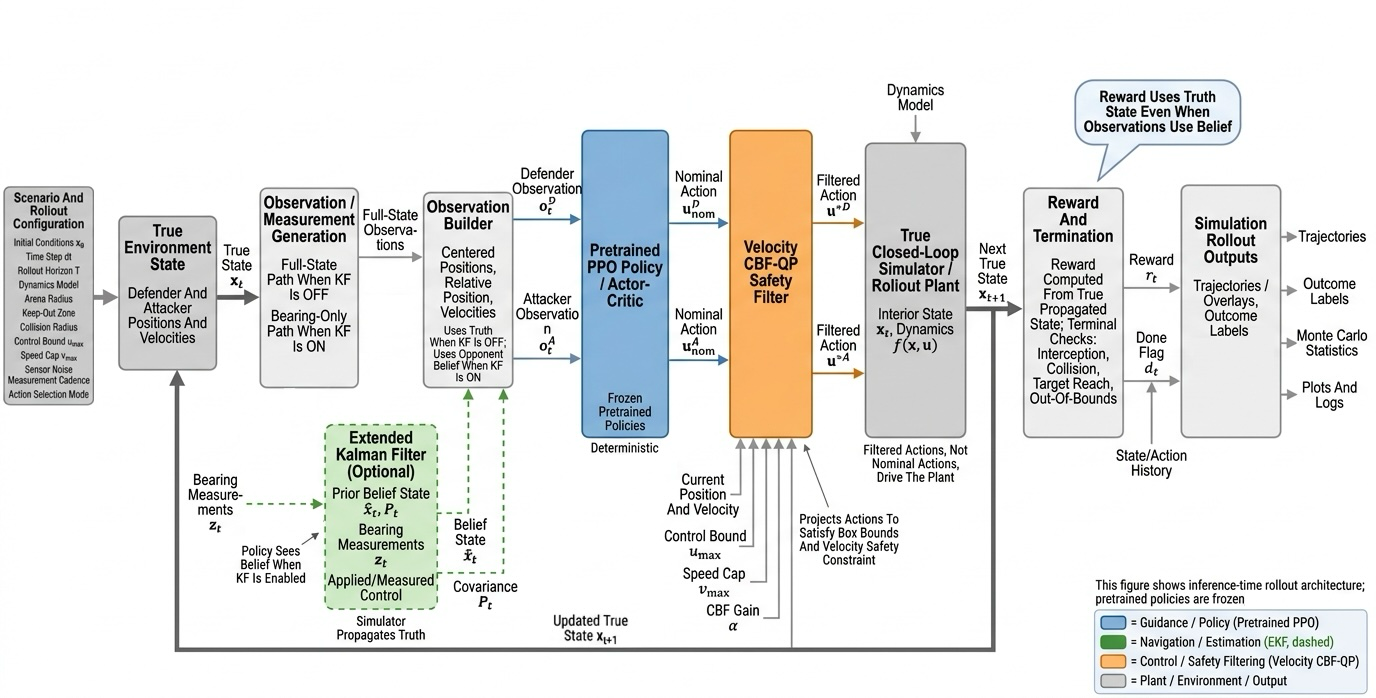
\includegraphics[width=1.0\linewidth]{Figures/Inference_Flattened.png}
    \caption{Diagram showing the inference process described in algorithm \ref{alg:actuation_interface}. A full-page version of this diagram is provided in Appendix~\ref{app:full_page_flowcharts} as Figure~\ref{fig:Inference_Flowchart_appendix}.}
    \label{fig:Inference_Flowchart}
\end{figure}
